%!TEX root = *.tex
%%%%%%%%%%%%%%%%%%
% カウンタのリセット
\setcounter{figure}{0}
% 問題文
以下の問いに答えなさい.

\hang{\ajRoman{1}.}
図1に示すように,質量が無視できて伸縮しない糸でつながれた2つの斜面の上に置かれている.
小物体の質量はともに$m$である.
糸は,なめらかに動く軽い低滑車にかけられ,
常に斜面と平行であるものとする.
左側の斜面が鉛直下方となす角は常に$60^\circ$であり,
右側の斜面が鉛直下方となす角$\theta\,(\theta>0^\circ)$は,変化させることができる.
斜面と糸は充分に長く,糸は,たるまないものとする.
なお,必要であれば,$\sqrt{2}\fallingdotseq 1.414$および$\sqrt{3}\fallingdotseq 1.732$を用いてもよい.

\sethang{\ajRoman{1}.} 
はじめに,小物体と斜面の間に摩擦力がはたらかない場合を考える.

\begin{enumerate}[(1)]
  \setlength{\leftskip}{-1.5zw}
  \setlength{\itemindent}{1zw}\setlength{\labelsep}{0.5zw}
  \setlength{\labelwidth}{1zw}\setlength{\leftmargin}{1zw}
  \setlength{\itemsep}{0.5\baselineskip}
  \item $\theta=60^\circ$に固定したとき,2つの小物体は静止していた.このときの糸の張力の大きさを,$g,\,m$を用いて表しなさい.
  \item $\theta$を,$0^\circ<\theta<60^\circ$をみたす値に固定したとき,2つの小物体を静止した状態から放すと,それぞれの小物体が,斜面に沿って同じ大きさ$a$の加速度で運動を始めた.運動を始めてから時間$t$の間に重力が2つの小物体にした仕事の和を,$a,\,m,\,t$を用いて表しなさい.
  \item (2)の運動において,$\theta=45^\circ$の場合,$\dfrac{a}{g}$の値を有効数字2桁で書き表しなさい.
\end{enumerate}

\sethang{\ajRoman{1}.}
つぎに,右側の小物体Aと斜面の間に摩擦力がはたらく場合を考える.
$\theta=60^\circ$で3つの小物体が斜面上に静止している状態から,
$\theta$をゆっくりと小さくしていったところ,$\theta=45^\circ$になった瞬間,
それぞれの小物体が,斜面に沿って同じ大きさ$a^\prime$の加速度で運動を始めた.
静止摩擦係数を$\mu\,(\mu>0)$,動摩擦係数を$\dfrac{\mu}{2}$とする.

\begin{enumerate}[(1)]
  \setlength{\leftskip}{-1.5zw}
  \setlength{\itemindent}{1zw}\setlength{\labelsep}{0.5zw}
  \setlength{\labelwidth}{1zw}\setlength{\leftmargin}{1zw}
  \setlength{\itemsep}{0.5\baselineskip}
  \addtocounter{enumi}{3}
  \item $\dfrac{a^\prime}{g}$の値を有効数字2桁で書き表しなさい.
\end{enumerate}

\hang{\ajRoman{2}.}
図2のように,質量$m$の小球が天井からゴムひもによりつり下げられており,
鉛直方向に運動するができる.
ゴムひもの自然長は$L$であり,その質量は無視できるものとする.
ゴムひもの長さが自然長より長いとき,
ばね定数を$k$とするフックの法則に従う復元力が小球にはたらくが,
たるんだ状態では,復元力ははたらかないものとする.
\z 軸の正の向きを鉛直上向きにとり,小球にはたらく重力とゴムひもによる復元力のつりあいの位置を$z=0$とする.
小球を鉛直下方に引き下げて静かに放すと,小球は\z 軸方向に運動した.
このとき,小球を放す位置が$-A\leqq z\leqq 0$($A$は正の定数)の場合のみ,小球は単振動した.
$z<-A$の位置で小球を静かに放すと,小球は単振動とは異なる運動を行った.
ゴムひもがたるんでいるとき,ゴムひもは小球の運動を妨げないものとする.
また,小球は天井に到達しないものとし,かつ\z 軸方向にのみ運動するものとする.

\begin{enumerate}[(1)]
  \setlength{\leftskip}{-1.5zw}
  \setlength{\itemindent}{1zw}\setlength{\labelsep}{0.5zw}
  \setlength{\labelwidth}{1zw}\setlength{\leftmargin}{1zw}
  \setlength{\itemsep}{0.5\baselineskip}
  \addtocounter{enumi}{4}
  \item $A$を$g,\,k,\,m$に用いて表しなさい.
  \item $z=-\dfrac{2mg}{k}$で小球を静かに放した後,小球が到達できる\z の最大値を,$g,\,k,\,m$を用いて表しなさい.
\end{enumerate}

\sethang{\ajRoman{2}.}
つぎに,小球のついたゴムひもを天井から取り外し,図3のように,水平面上の点Oにつないだ.
点Oを中心として,小球を速さ$v$で等速円運動させた.
小球が等速円運動しているとき,ゴムひもの自然長からの伸びを$x\,(x>0)$とする.
小球と水平面の間に摩擦はなく,ゴムひもは,ねじれないものとする.

\begin{enumerate}[(1)]
  \setlength{\leftskip}{-1.5zw}
  \setlength{\itemindent}{1zw}\setlength{\labelsep}{0.5zw}
  \setlength{\labelwidth}{1zw}\setlength{\leftmargin}{1zw}
  \setlength{\itemsep}{0.5\baselineskip}
  \addtocounter{enumi}{6}
  \item 等速円運動の周期を,$v,\,L,\,x$を用いて表しなさい.
  \item 小球の速さ$v$を,$k,\,m,\,L,\,x$を用いて表しなさい.
  \item 小球の運動エネルギーは,ゴムひもの弾性エネルギー(弾性力による位置エネルギー)の何倍か,$L,\,x$を用いて表しなさい.ただし,$x=0$のときのゴムひもの弾性エネルギーを0とする.
\end{enumerate}


\begin{figure}[H]
  \centering
  \begin{minipage}[b]{.45\columnwidth}
    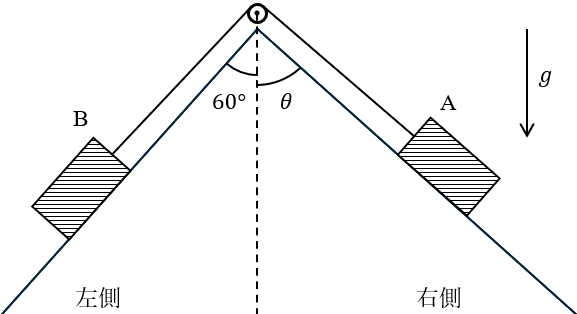
\includegraphics[width=\columnwidth]{../graphs/toritsu_23_1-1.png}
    \caption{}
  \end{minipage}
  \begin{minipage}[b]{.25\columnwidth}
    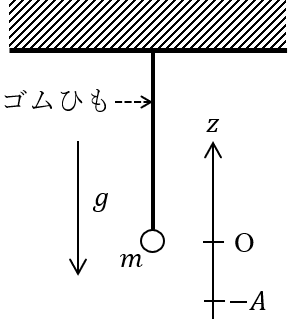
\includegraphics[width=\columnwidth]{../graphs/toritsu_23_1-2.png}
    \caption{}
  \end{minipage}
  \begin{minipage}[b]{.25\columnwidth}
    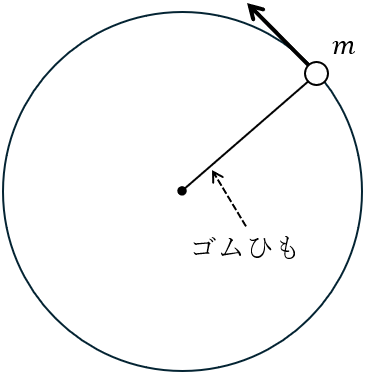
\includegraphics[width=\columnwidth]{../graphs/toritsu_23_1-3.png}
    \caption{}
  \end{minipage}
\end{figure}

% メモ
\begin{comment}

\end{comment}


%%%%%%%%%%%%%%%%%%
